\documentclass[12pt, git, final]{rureport}


\begin{document} % this tells the compiler that it is time to make
                 % text to print instead of just getting ready.
\maketitle  % make a title page from the Title, Date, and Author

%\fxnote{skoða titil á skýrslu, sbr. forsíðu}

%\section*{Errata} %%section* avoids putting a number 
%
\section{Inngangur} % sections break up the document into pieces
Himingeimurinn er fyrir mörgum jafn áhugaverður og hann er að stærð og menn hafa öldum saman spáð mikið í himintunglum og önnur fyrirbæri út í geimi. Ákveðið var því að ná í gögn fyrir sólmyrkva jarðar, ásamt því að ná í gögn fyrir stríð  sem herjað hefur jörðina og vopnasölu út um heim allan. Fyrst og fremst vildi hópurinn skoða hvernig stríð dreifist á jörðina, hversu oft og hvar lenda sólmyrkvarnari á jörðina meðan stríðin geisa og hvort það sé möguleiki á fylgni milli fjölda sólmyrkva og fjölda stríðsátaka? Þessir útgangspunktar verða skoðaðir nánar og gefin frekari skil á niðurstöðunum.  
\section{Framkvæmd}
\subsection{Hnötturinn}
Við gerð hnattarins þá var notast við Basemap sem er viðbót við matplotlib, til að búa til jörðina þá er notað fall sem tekur inn lönd, lengdar og breiddarbauga sem 'ints' og plottar, síðan er hnötturinn gerður raunverulegri með innbyggðu falli sem heitir map.bluemarble(). Notast var við gögn úr gagnagrunninum til að fá hnit sólmyrkvana frá 1901-2100 og til að framkalla svo snúning jarðarinnar þá búnar til 180 myndir á tveggja lengdargráðu fresti, því næst er nota Image sequence clip pakkan \cite{moviepy} fyrir python sem býr til hreyfimynd.
 
\subsection{Myndrænt notendaviðmót}



\section{Aðferð}
\subsection{Gögn}
Fyrst var farið á veraldarvefin og leitað af gögnum sem hægt væri að vinna með, gögnin voru fundin á síðu á síðu hjá NASA \cite{Eclipse}, Stockholm international peace research institution \cite{weapon} og Háskólanum í Uppsölum í Svíþjóð \cite{conflict}. Gögnin voru tekin inn á csv formi, þau voru svo hreinsuð í python og unnið með þau sem Dataframes.
\subsection{Hönnun}
Við hönnun á GUI þá notast  við Qt4 Designer \cite{qt4}. Ákveðið var að það yrði innskráningar gluggi (sjá mynd \ref{fig:logScreen}) og þar þarf að skrá inn upplýsingar til að tengjast gagnagrunninum og nota notendaviðmótið sem lætur vita hvort tenging hafi heppnast eða mispheppnast ( sjá mynd \ref{fig:logsucces}) 

Við notumst við Basemap\cite{basemap} sem er viðbótarpakki fyrir Matplotlib til að sýna hvernig sólmyrkvinn lendir á jörðinni. Gögnin um sólmyrkvan eru frá NASA og eru þær upplýsingar notaðar til að sýna staðsetningarnar sólmyrkvana á jörðinni, einnig sýnum við að 

\subsection{Virkni forrits}
Eftir að notandi er búinn að tengjast gagnagrunni þá getur hann skoðar ýmsar upplýsingar út frá árum. Það er hægt að hreyfa við stiku til að fá árið af eigin vali eða slegið inn ártalið til að fá viðkomandi upplýsingar um hvað gerðist á því ári til að fá upp upplýsingar eftir hentisemi, upplýsingarnar skila sér svo á kortinu sem er á upphafskjánnum og það birtast upplýsingar í dálkum vinstra megin fyrir. 


\section{Niðurstöður}\label{nidurstodur}
Hópurinn
Þegar plottaðir voru staðsetningarnar fyrir sólmyrkvana þá sást að lína myndaðist á breiddargráðum 60$^{\circ}$-75$^{\circ}$ bæði á norður- (sjá mynd \ref{fig:3DNP}) og suðurhveli (sjá mynd \ref{fig:3DSP}) og sú lína spannar ca 43,6\% af öllum sólmyrkvunum sem hafa verið á jörðinni frá tímabilinu 1901 - 2100. Hægt er að sjá að á svæðum sem sólmyrkvarnir mynda þéttan kjarna, því færri stríð hafa geisað á þeim svæðum sbr 60$^{\circ}$-75$^{\circ}$
\pagebreak

\begin{figure}
	\centering
	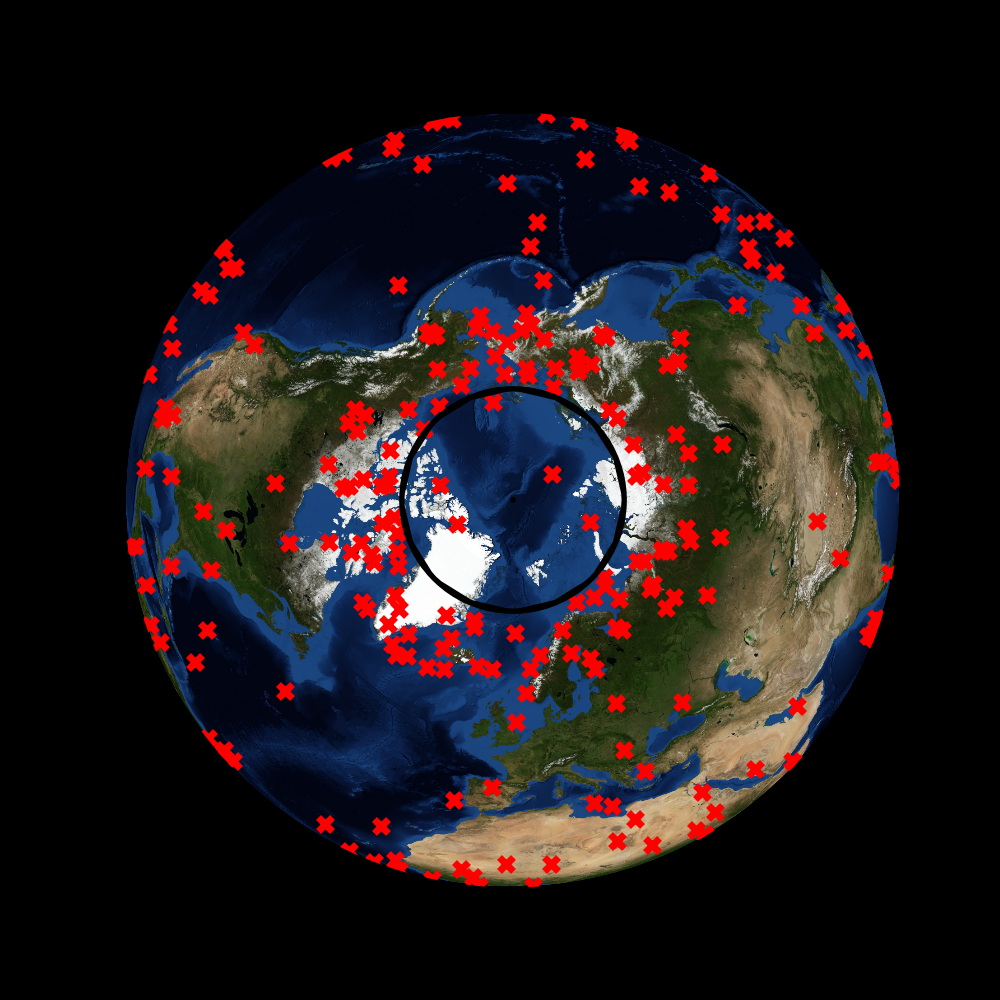
\includegraphics[width=10cm]{3DNP.png}
	\caption{Sólmyrkvarnir séð frá Norður pólnum}
	\label{fig:3DNP}
\end{figure}

\begin{figure}
	\centering
	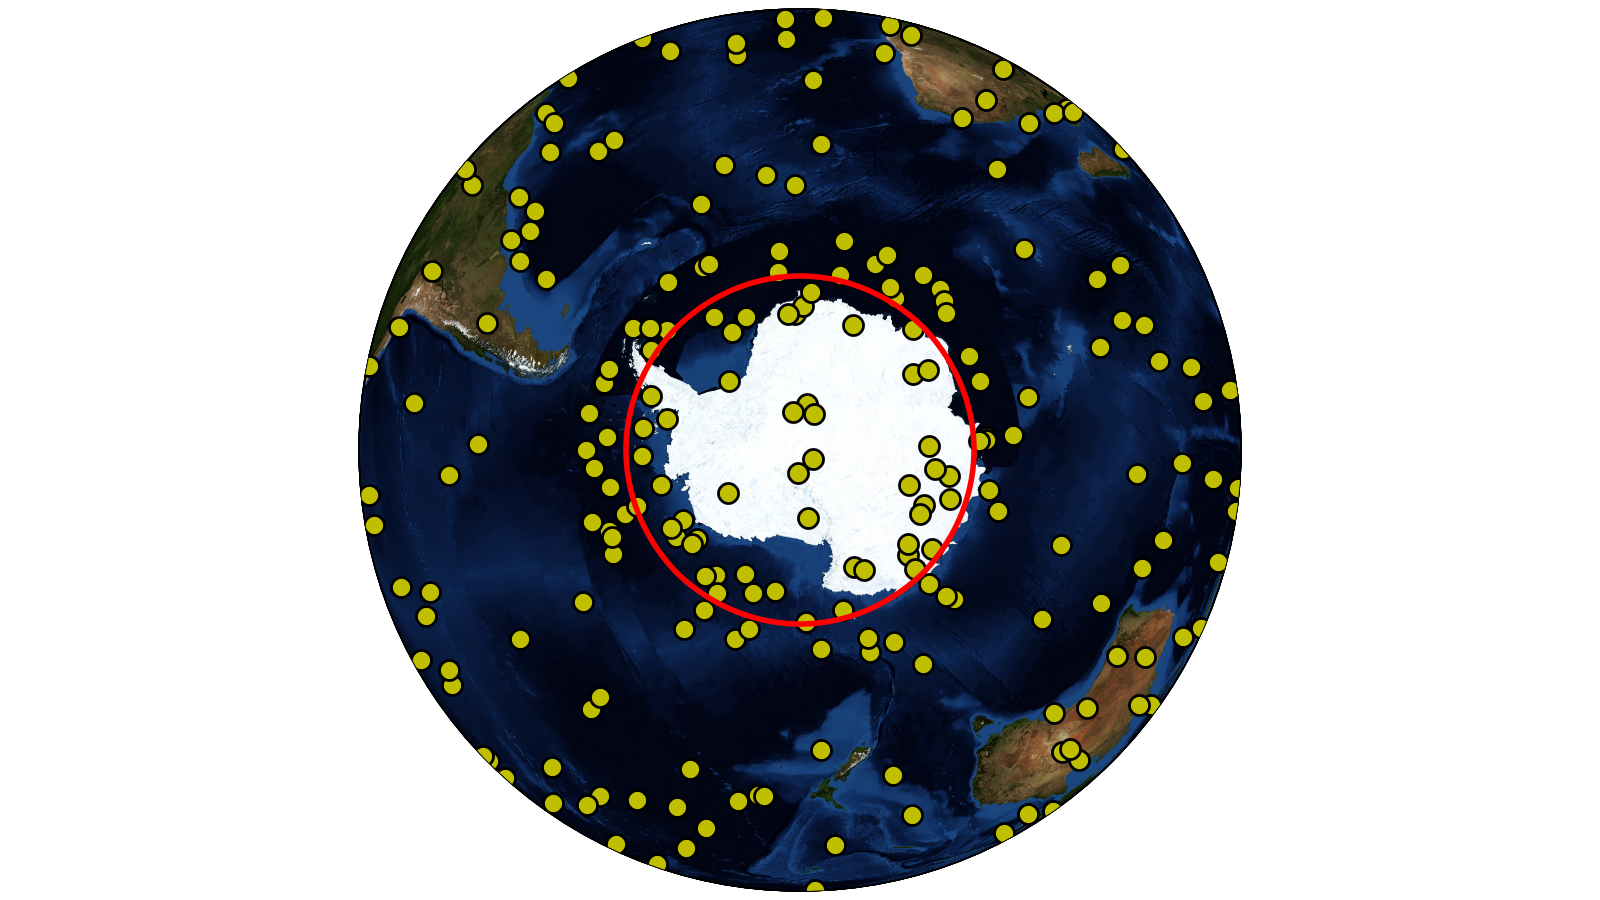
\includegraphics[width=10cm]{3DSP.png}
	\caption{Sólmyrkvarnir séð frá Suður pólnum}
	\label{fig:3DSP}
\end{figure}

\begin{figure}
	\centering 
	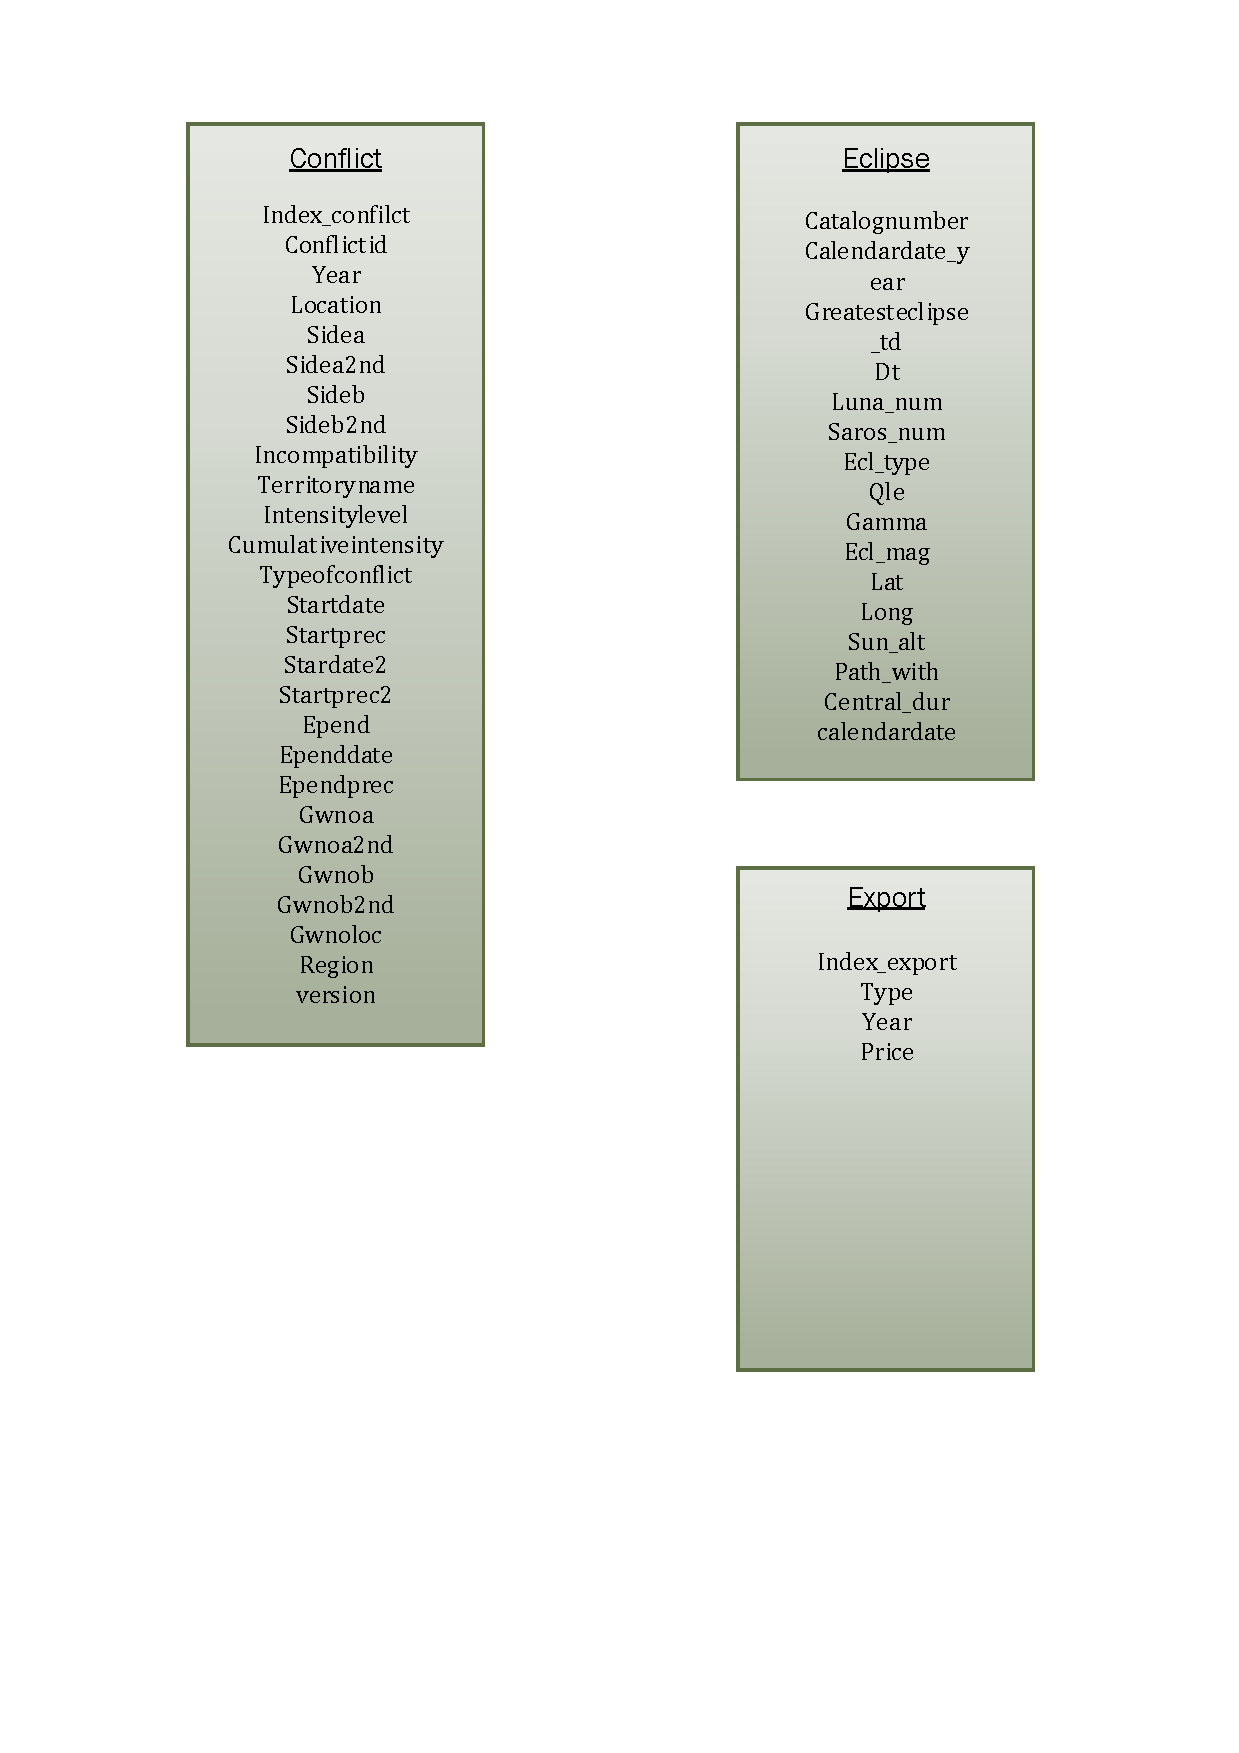
\includegraphics[width = 18cm]{dataSchema.pdf}
	\caption{Database schema \label{fig:dataschema}}
\end{figure} 
%
\begin{figure}
	\centering 
	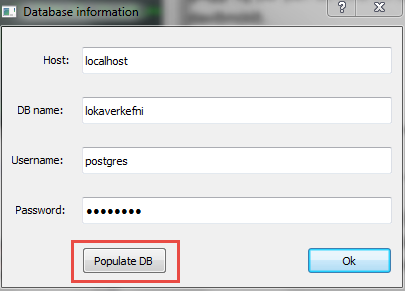
\includegraphics[width = 8cm]{logInScreen.png}
	\caption{Database schema \label{fig:logScreen}}
\end{figure} 

\begin{figure}
	\centering 
	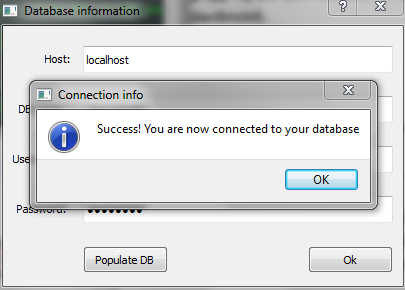
\includegraphics[width = 8cm]{logInSuccess.png}
	\caption{Database schema \label{fig:logsucces}}
\end{figure} 

\begin{figure}[t]
	\centering 
	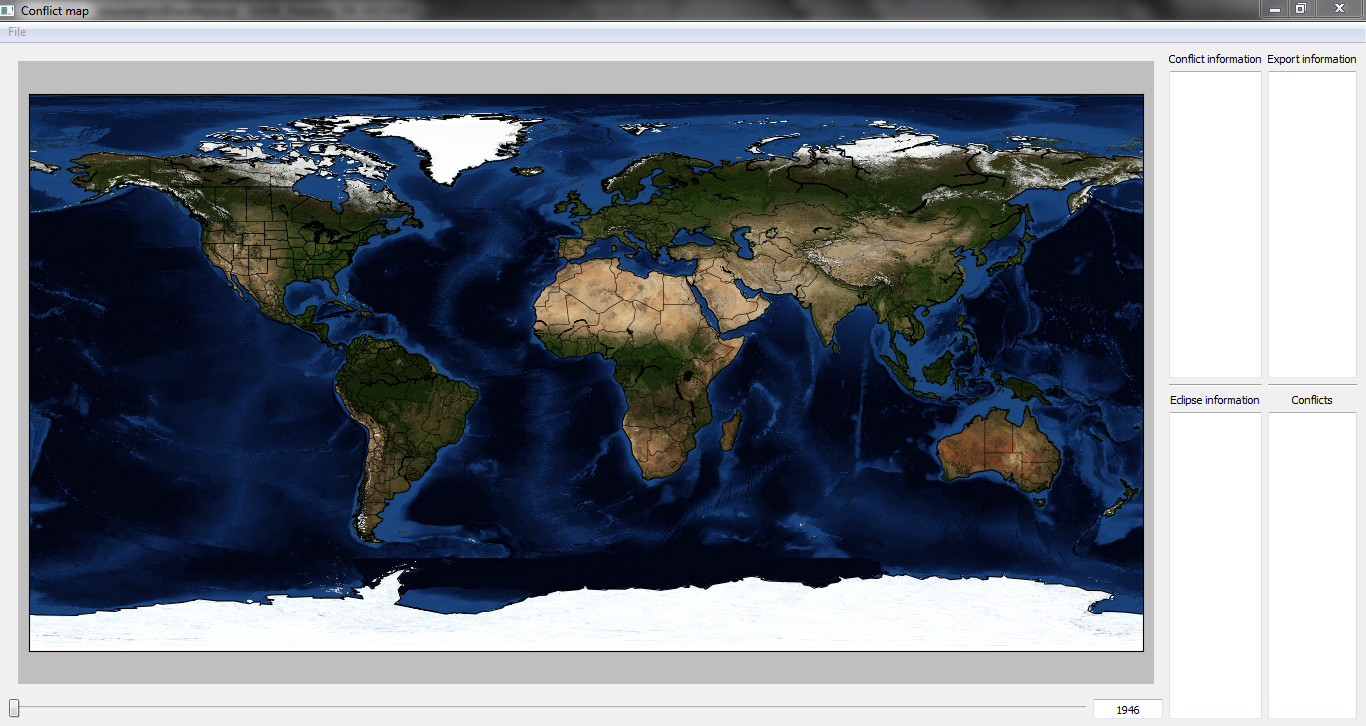
\includegraphics[width = 18cm]{openScreen.png}
	\caption{Database schema \label{fig:openScreen}}
\end{figure} 

\clearpage

\printbibliography

\end{document} % this tells the compiler that we are done

% These are variables for the editor Emacs
%%% Local Variables: 
%%% TeX-command-BibTeX: biber
%%% mode: latex
%%% TeX-master: t
%%% End:
